\documentclass[a4paper, 11pt, titlepage]{report}
\usepackage{graphicx}
\usepackage{fullpage}
\usepackage{float}
%\usepackage{longtable}
\usepackage{amsmath}
%\usepackage[normalem]{ulem}
\usepackage{booktabs}
%\usepackage{array}
%\usepackage{tikz}
%\usepackage{parskip}
%\newcommand{\tabitem}{~~\llap{\textbullet}~~}
\setlength{\tabcolsep}{18pt}
\renewcommand{\arraystretch}{1.5}
\renewcommand{\chaptername}{Study Unit}
\usepackage[dvipsnames]{xcolor}
\usepackage{hyperref}
\hypersetup{
    colorlinks=true,
    linkcolor=RoyalBlue,
    filecolor=magenta,
    urlcolor=RoyalBlue,
    citecolor=RoyalBlue
}
\begin{document}
\linespread{1.25}
\title{CMPG321 - Advanced Databases\\Additional Notes\\Semester 2}
\date{}
\maketitle
\tableofcontents{}

\chapter{Transaction Management and Concurrency Control}
\section{What Is a Transaction?}
A \textbf{transaction} is a \textit{logical} unit of work that must be entirely completed or entirely aborted; no intermediate states are acceptable.\\
A \textbf{consistent database state} is one in which all data integrity constraints are satisfied. To ensure consistency of the database, every transaction must begin with the database in a known consistent state.
\subsection{Evaluating Transaction Results}
Not all transactions update the database. The DBMS cannot guarantee that the semantic meaning of the transaction truly represents the real-world event.
\subsection{Transaction Properties}
Each individual transaction must display atomicity, consistency, isolation, and durability.
These four properties are sometimes referred to as the ACID test.
\begin{itemize}
\item \textit{Atomicity} requires that all operations (SQL requests) of a transaction be completed;
if not, the transaction is aborted.
\item \textit{Consistency} indicates the permanence of the database's consistent state. A transaction takes a database from one consistent state to another. When a transaction is completed, the database must be in a consistent state. If any of the transaction parts violates an integrity constraint, the entire transaction is aborted.
\item \textit{Isolation} means that the data used during the execution of a transaction cannot be used by a second transaction until the first one is completed.
\item \textit{Durability} ensures that once transaction changes are done and committed, they cannot be undone or lost, even in the event of a system failure.
\end{itemize}
\subsection{Transaction Management with SQL}
\begin{itemize}
\item When a \texttt{COMMIT} statement is reached, all changes are permanently recorded within the database. The \texttt{COMMIT} statement automatically ends the SQL transaction.
\item When a \texttt{ROLLBACK} statement is reached, all changes are aborted and the database is rolled back to its previous consistent state.
\item The end of a program is successfully reached, in which case all changes are permanently recorded within the database. This action is equivalent to \texttt{COMMIT}.
\item The program is abnormally terminated, in which case the database changes are aborted and the database is rolled back to its previous consistent state. This action is equivalent to \texttt{ROLLBACK}.
\end{itemize}
\subsection{The Transaction Log}
A DBMS uses a \textbf{transaction log} to keep track of all transactions that update the database. The DBMS uses the information stored in this log for a recovery requirement triggered by a \texttt{ROLLBACK} statement, a program's abnormal termination, or a system failure such as a network discrepancy or a disk crash. Some RDBMSs use the transaction log to recover a database forward to a currently consistent state.

While the DBMS executes transactions that modify the database, it also automatically updates the transaction log. The transaction log stores the following:
\begin{itemize}
\item A record for the beginning of the transaction.
\item For each transaction component (SQL statement):
\begin{itemize}
\item The type of operation being performed (\texttt{INSERT}, \texttt{UPDATE}, \texttt{DELETE}).
\item The names of the objects affected by the transaction (the name of the table).
\item The \textit{"before"} and \textit{"after"} values for the fields being updated.
\item Pointers to the previous and next transaction log entries for the same transaction.
\end{itemize}
\item The ending (\texttt{COMMIT}) of the transaction.
\end{itemize}
\section{Concurrency Control}
Coordinating the simultaneous execution of transactions in a multiuser database system is known as \textbf{concurrency control}. The objective of concurrency control is to ensure the serializability of transactions in a multiuser database environment. To achieve this goal, most concurrency control techniques are oriented toward preserving the isolation property of concurrently executing transactions. Concurrency control is important because the simultaneous execution of transactions over a shared database can create several data integrity and consistency problems. The three main problems are lost updates, uncommitted data, and inconsistent retrievals.
\subsection{Lost Updates}
The \textbf{lost update} problem occurs when two concurrent transactions, T1 and T2, are updating the same data element and one of the updates is lost (overwritten by the other transaction).
\subsection{Uncommitted Data}
The phenomenon of \textbf{uncommitted data} occurs when two transactions, T1 and T2, are executed concurrently and the first transaction (T1) is rolled back after the second transaction (T2) has already accessed the uncommitted data—thus violating the isolation property of transactions.
\subsection{Inconsistent Retrievals}
\textbf{Inconsistent retrievals} occur when a transaction accesses data before and after one or more other transactions finish working with such data. For example, an inconsistent retrieval would occur if transaction T1 calculated some summary (aggregate) function over a set of data while another transaction (T2) was updating the same data. The problem is that the transaction might read some data before it is changed and other data after it is changed, thereby yielding inconsistent results.
\subsection{The Scheduler}
The \textbf{scheduler} is a special DBMS process that establishes the order in which the operations are executed within concurrent transactions. The scheduler \textit{interleaves} the execution of database operations to ensure serializability and isolation of transactions. To determine the appropriate order, the scheduler bases its actions on concurrency control algorithms, such as locking or time stamping methods.

The scheduler's main job is to create a serializable schedule of a transaction's operations, in which the interleaved execution of the transactions (T1, T2, T3, etc.) yields the same results as if the transactions were executed in serial order (one after another).

The scheduler also makes sure that the computer's central processing unit (CPU) and
storage systems are used efficiently.
\section{Concurrency Control with Locking Methods}
 A \textbf{lock} guarantees exclusive use of a data item to a current transaction. In other words, transaction T2 does not have access to a data item that is currently being used by transaction T1. A transaction acquires a lock prior to data access; the lock is released (unlocked) when the transaction is completed.

The use of locks based on the assumption that conflict between transactions is likely is usually referred to as \textbf{pessimistic locking}.

Most multiuser DBMSs automatically initiate and enforce locking procedures. All lock information is handled by a \textbf{lock manager}, which is responsible for assigning and policing the locks used by the transactions.
\subsection{Lock Granularity}
\textbf{Lock granularity} indicates the level of lock use. Locking can take place at the following levels: database, table, page, row, or even field (attribute).\\\\
\textit{Database Level} - In a \textbf{database-level lock}, the entire database is locked, thus preventing the use of any tables in the database by transaction T2 while transaction T1 is being executed. This level of locking is good for batch processes, but it is unsuitable for multiuser DBMSs. Transactions T1 and T2 cannot access the same database concurrently \textit{even when they use different tables}.\\\\
\textit{Table Level} - In a \textbf{table-level lock}, the entire table is locked, preventing access to any row by transaction T2 while transaction T1 is using the table. If a transaction requires access to several tables, each table may be locked. However, two transactions can access the same database as long as they access different tables. Table-level locks, while less restrictive than database-level locks, cause traffic jams when many transactions are waiting to access the same table.\\\\
\textit{Page Level} - In a \textbf{page-level lock}, the DBMS locks an entire \textbf{diskpage}. A diskpage, or page, is the equivalent of a \textit{diskblock}, which can be described as a directly addressable section of a disk. A page has a fixed size, such as 4K, 8K, or 16K. For example, if you want to write only 73 bytes to a 4K page, the entire 4K page must be read from disk, updated in memory, and written back to disk. A table can span several pages, and a page can contain several rows of one or more tables. Page-level locks are currently the most frequently used locking method for multiuser DBMSs.\\\\
\textit{Row Level} - A \textbf{row-level lock} is much less restrictive than the locks discussed earlier.
The DBMS allows concurrent transactions to access different rows of the same table even when the rows are located on the same page. Although the row-level locking approach improves the availability of data, its management requires high overhead because a lock exists for each row in a table of the database involved in a conflicting transaction. Modern DBMSs automatically escalate a lock from a row level to a page level when the application session requests multiple locks on the same page.\\\\
\textit{Field Level} - The \textbf{field-level lock} allows concurrent transactions to access the same row as long as they require the use of different fields (attributes) within that row. Although field-level locking clearly yields the most flexible multiuser data access, it is rarely implemented in a DBMS because it requires an extremely high level of computer overhead and because the row-level lock is much more useful in practice.
\subsection{Lock Types}
\textit{Binary} - A \textbf{binary lock} has only two states: locked (1) or unlocked (0). If an object such as a database, table, page, or row is locked by a transaction, no other transaction can use that object. If an object is unlocked, any transaction can lock the object for its use. Every database operation requires that the affected object be locked. As a rule, a transaction must unlock the object after its termination. Therefore, every transaction requires a lock and unlock operation for each accessed data item. Such operations are automatically managed and scheduled by the DBMS.\\\\
\textit{Shared/Exclusive} - An \textbf{exclusive lock} exists when access is reserved specifically for the transaction that locked the object. The exclusive lock must be used when the potential for conflict exists. A \textbf{shared lock} exists when concurrent transactions are granted read access on the basis of a common lock. A shared lock produces no conflict as long as all the concurrent transactions are read-only.
Two transactions conflict only when at least one is a write transaction. Because the two read transactions can be safely executed at once, shared locks allow several read transactions to read the same data item concurrently. For example, if transaction T1 has a shared lock on data item X and transaction T2 wants to read data item X, T2 may also obtain a shared lock on data item X. If transaction T2 updates data item X, an exclusive lock is required by T2 over data item X. The exclusive lock is granted if and only if no other locks are held on the data item (this condition is known as the \textbf{mutual exclusive rule}: only one transaction at a time can own an exclusive lock on an object.) Therefore, if a shared (or exclusive) lock is already held on data item X by transaction T1, an exclusive lock cannot be granted to transaction T2, and T2 must wait to begin until T1 commits. In other words, a
shared lock will always block an exclusive (write) lock; hence, decreasing transaction concurrency.\\\\
Although the use of shared locks renders data access more efficient, a shared/exclusive
lock schema increases the lock manager's overhead for several reasons:
\begin{itemize}
\item The type of lock held must be known before a lock can be granted.
\item Three lock operations exist: \texttt{READ\_LOCK} to check the type of lock, \texttt{WRITE\_LOCK} to issue the lock, and \texttt{UNLOCK} to release the lock.
\item The schema has been enhanced to allow a lock upgrade from shared to exclusive and a lock downgrade from exclusive to shared.
Although locks prevent serious data inconsistencies, they can lead to two major problems:
\begin{itemize}
\item The resulting transaction schedule might not be serializable.
\item The schedule might create deadlocks. A \textbf{deadlock} occurs when two transactions wait indefinitely for each other to unlock data. A database deadlock, which is similar to traffic gridlock in a big city, is caused when two or more transactions wait for each other to unlock data.
\end{itemize}
Fortunately, both problems can be managed: serializability is attained through a locking protocol known as two-phase locking, and deadlocks can be managed by using deadlock detection and prevention techniques.
\end{itemize}
\subsection{Two-Phase Locking to Ensure Serializability}
\textbf{Two-phase locking} (2PL) defines how transactions acquire and relinquish locks. Two-phase locking guarantees serializability, but it does not prevent deadlocks. The two phases are:
\begin{enumerate}
\item A growing phase, in which a transaction acquires all required locks without unlocking any data. Once all locks have been acquired, the transaction is in its locked point.
\item A shrinking phase, in which a transaction releases all locks and cannot obtain a new lock.
\end{enumerate}
The two-phase locking protocol is governed by the following rules:
\begin{itemize}
\item Two transactions cannot have conflicting locks.
\item No unlock operation can precede a lock operation in the same transaction.
\item No data is affected until all locks are obtained—that is, until the transaction is in its
locked point.
\end{itemize}
\begin{figure}[H]
\centering
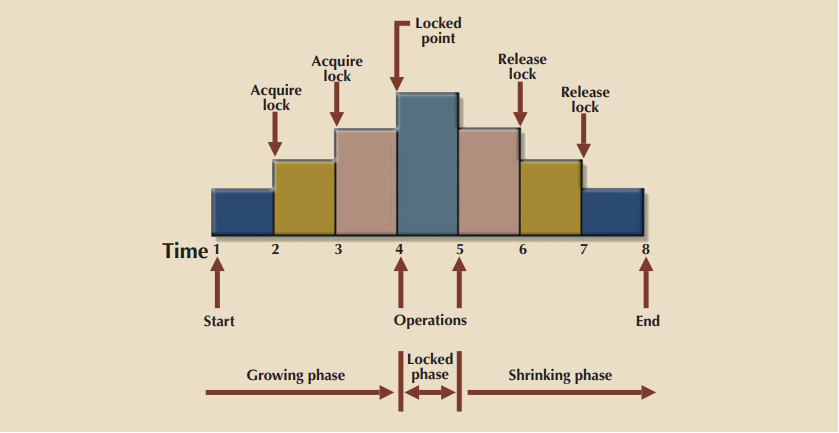
\includegraphics[scale=0.75]{pics/lock}
\caption{Two-phase locking process illustrated}
\end{figure}
\subsection{Deadlocks}
A deadlock occurs when two transactions wait indefinitely for each other to unlock data. For
example, a deadlock occurs when two transactions, T1 and T2, exist in the following mode:
\begin{center}
T1 = access data items X and Y\\
T2 = access data items Y and X
\end{center}
If T1 has not unlocked data item Y, T2 cannot begin; if T2 has not unlocked data item X, T1 cannot continue. Consequently, T1 and T2 each wait for the other to unlock the required data item. Such a deadlock is also known as a \textbf{deadly embrace}. Note that deadlocks are possible only when one of the transactions wants to obtain an exclusive lock on a data item; no deadlock condition can exist among \textit{shared} locks.

The three basic techniques to control deadlocks are:
\begin{itemize}
\item \textit{Deadlock prevention}. A transaction requesting a new lock is aborted when there is the possibility that a deadlock can occur. If the transaction is aborted, all changes made by this transaction are rolled back and all locks obtained by the transaction are released. The transaction is then rescheduled for execution. Deadlock prevention works because it avoids the conditions that lead to deadlocking.
\item \textit{Deadlock detection}. The DBMS periodically tests the database for deadlocks. If a deadlock is found, the "victim" transaction is aborted (rolled back and restarted) and the other transaction continues.
\item \textit{Deadlock avoidance}. The transaction must obtain all of the locks it needs before it can be executed. This technique avoids the rolling back of conflicting transactions by requiring that locks be obtained in succession. However, the serial lock assignment required in deadlock avoidance increases action response times.
\end{itemize}
\section{Concurrency Control with Time Stamping Methods}
The \textbf{time stamping} approach to scheduling concurrent transactions assigns a global, unique time stamp to each transaction. The time stamp value produces an explicit order in which transactions are submitted to the DBMS. Time stamps must have two properties: uniqueness and monotonicity. \textbf{Uniqueness} ensures that no equal time stamp values can exist, and \textbf{monotonicity}\footnote{The term monotonicity is part of the standard concurrency control vocabulary.} ensures that time stamp values always increase.
\subsection{Wait/Die and Wound/Wait Schemes}
Using the wait/die scheme:
\begin{itemize}
\item If the transaction requesting the lock is the older of the two transactions, it will wait until the other transaction is completed and the locks are released.
\item If the transaction requesting the lock is the younger of the two transactions, it will die (roll back) and is rescheduled using the same time stamp.
\end{itemize}
In short, in the \textbf{wait/die} scheme, the older transaction waits for the younger one to complete and release its locks.
In the wound/wait scheme:
\begin{itemize}
\item If the transaction requesting the lock is the older of the two transactions, it will \textit{preempt (wound)} the younger transaction by rolling it back. T1 preempts T2 when T1 rolls back T2. The younger, preempted transaction is rescheduled using the same time stamp.
\item If the transaction requesting the lock is the younger of the two transactions, it will wait until the other transaction is completed and the locks are released.
\end{itemize}
In short, in the \textbf{wound/wait} scheme, the older transaction rolls back the younger transaction and reschedules it. In both schemes, one of the transactions waits for the other transaction to finish and
release the locks.
\section{Concurrency Control with Optimistic Methods}
The \textbf{optimistic approach} is based on the assumption that the majority of database operations do not conflict. The optimistic approach requires neither locking nor time stamping techniques. Instead, a transaction is executed without restrictions until it is committed. Using an optimistic approach, each transaction moves through two or three phases, referred to as \textit{read}, \textit{validation}, and \textit{write}.
\begin{itemize}
\item During the \textit{read phase}, the transaction reads the database, executes the needed computations, and makes the updates to a private copy of the database values. All update operations of the transaction are recorded in a temporary update file, which is not accessed by the remaining transactions.
\item During the \textit{validation phase}, the transaction is validated to ensure that the changes made will not affect the integrity and consistency of the database. If the validation test is positive, the transaction goes to the write phase. If the validation test is negative, the transaction is restarted and the changes are discarded.
\item During the \textit{write phase}, the changes are permanently applied to the database.
\end{itemize}
\section{Database Recovery Management}
\textbf{Database recovery} restores a database from a given state (usually inconsistent) to a previously consistent state. Recovery techniques are based on the \textbf{atomic transaction property}: all portions of the transaction must be treated as a single, logical unit of work in which all operations are applied and completed to produce a consistent database.

Critical events can cause a database to stop working and compromise the integrity of the data. Examples of critical events are:
\begin{itemize}
\item \textit{Hardware/software failures}. A failure of this type could be a hard disk media failure,
a bad capacitor on a motherboard, or a failing memory bank. Other causes of errors under this category include application program or operating system errors that cause data to be overwritten, deleted, or lost.
\item \textit{Human-caused incidents}. This type of event can be categorized as unintentional or
intentional.
\begin{itemize}
\item An unintentional failure is caused by a careless end user. Such errors include deleting the wrong rows from a table, pressing the wrong key on the keyboard, or shutting down the main database server by accident.
\item Intentional events are of a more severe nature and normally indicate that the company data is at serious risk. Under this category are security threats caused by hackers trying to gain unauthorized access to data resources and virus attacks caused by disgruntled employees trying to compromise the database operation and damage the company.
\end{itemize}
\item \textit{Natural disasters}. This category includes fires, earthquakes, floods, and power failures.
\end{itemize}
\subsection{Transaction Recovery}
Database transaction recovery uses data in the transaction log to recover a database from an inconsistent state to a consistent state.There are four important concepts that affect the recovery process:
\begin{itemize}
\item The \textbf{write-ahead-log protocol} ensures that transaction logs are always written before
any database data is actually updated.
\item \textbf{Redundant transaction logs} ensure that a physical disk failure will not impair the DBMS's ability to recover data.
\item Database \textbf{buffers} are temporary storage areas in primary memory used to speed up
disk operations. To improve processing time, the DBMS software reads the data from the physical disk and stores a copy of it on a "buffer" in primary memory.
\item Database \textbf{checkpoints} are operations in which the DBMS writes all of its updated buffers in memory (also known as \textit{dirty buffers}) to disk. While this is happening, the DBMS does not execute any other requests. A checkpoint operation is also registered in the transaction log. As a result of this operation, the physical database and the transaction log will be in sync.
\end{itemize}
The database recovery process involves bringing the database to a consistent state
after a failure. Transaction recovery procedures generally make use of deferred-write and
write-through techniques.

When the recovery procedure uses a \textbf{deferred-write technique} (also called a \textbf{deferred update}), the transaction operations do not immediately update the physical database. Instead, only the transaction log is updated. The database is physically updated only with data from committed transactions, using information from the transaction log. If the transaction aborts before it reaches its commit point, no changes (no \texttt{ROLLBACK} or undo) need to be made to the database because it was never updated. The recovery process for all started and committed transactions (before the failure) follows these steps:
\begin{enumerate}
\item Identify the last checkpoint in the transaction log. This is the last time transaction data was physically saved to disk.
\item For a transaction that started and was committed before the last checkpoint, nothing needs to be done because the data is already saved.
\item For a transaction that performed a commit operation after the last checkpoint, the DBMS uses the transaction log records to redo the transaction and update the database, using the "after" values in the transaction log. The changes are made in ascending order, from oldest to newest.
\item For any transaction that had a \texttt{ROLLBACK} operation after the last checkpoint or
that was left active (with neither a \texttt{COMMIT} nor a \texttt{ROLLBACK}) before the failure
occurred, nothing needs to be done because the database was never updated.
\end{enumerate}
When the recovery procedure uses a \textbf{write-through technique} (also called an
\textbf{immediate update}), the database is immediately updated by transaction operations during
the transaction's execution, even before the transaction reaches its commit point. If the transaction aborts before it reaches its commit point, a \texttt{ROLLBACK} or undo operation needs to
be done to restore the database to a consistent state. In that case, the \texttt{ROLLBACK} operation
will use the transaction log "before" values. The recovery process follows these steps:
\begin{enumerate}
\item Identify the last checkpoint in the transaction log. This is the last time transaction
data was physically saved to disk.
\item For a transaction that started and was committed before the last checkpoint, nothing
needs to be done because the data is already saved.
\item For a transaction that was committed after the last checkpoint, the DBMS re-does
the transaction, using the "after" values of the transaction log. Changes are applied in
ascending order, from oldest to newest.
\item For any transaction that had a \texttt{ROLLBACK} operation after the last checkpoint or that was left active (with neither a \texttt{COMMIT} nor a \texttt{ROLLBACK}) before the failure occurred, the DBMS uses the transaction log records to \texttt{ROLLBACK} or undo the operations, using the "before" values in the transaction log. Changes are applied in reverse order, from newest to oldest.
\end{enumerate}
\chapter{Database Performance Tuning and Query Optimization}
\section{Database Performance-Tuning Concepts}
One of the main functions of a database system is to provide timely answers to end users. End users interact with the DBMS through the use of queries to generate information, using the following sequence:
\begin{enumerate}
\item The end-user (client-end) application generates a query.
\item The query is sent to the DBMS (server end).
\item The DBMS (server end) executes the query.
\item The DBMS sends the resulting data set to the end-user (client-end) application.
\end{enumerate}
\textbf{Database performance tuning} refers to a set of activities and procedures designed to reduce the response time of the database system-that is, to ensure that an end-user query is processed by the DBMS in the minimum amount of time.
\begin{center}
\textbf{Good database performance starts with good database design}. \textit{No amount of fine tuning will make a poorly designed database perform as well as a well-designed database}. 
\end{center}
\subsection{Performance Tuning: Client and Server}
In general, database performance-tuning activities can be divided into those on the client side and those on the server side.

On the client side, the objective is to generate a SQL query that returns the correct answer in the least amount of time, using the minimum amount of resources at the server end. The activities required to achieve that goal are commonly referred to as \textbf{SQL performance tuning}.

On the server side, the DBMS environment must be properly configured to respond to clients' requests in the fastest way possible, while making optimum use of existing resources. The activities required to achieve that goal are commonly referred to as \textbf{DBMS performance tuning}.
\subsection{DBMS Architecture}
\begin{figure}[H]
\centering
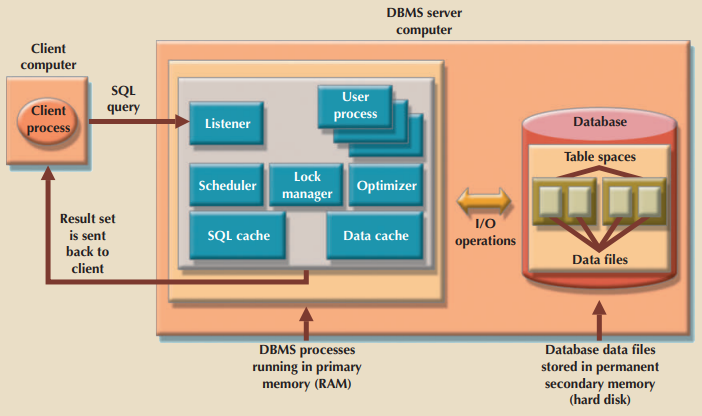
\includegraphics[scale=0.6]{pics/arch}
\caption{DBMS Architecture}
\end{figure}
All data in a database is stored in \textbf{data files}. A data file can contain rows from a single table, or it can contain rows from many different tables. Data files can automatically expand as required in predefined increments known as \textbf{extents}.

Data files are generally grouped in file groups or table spaces. A \textbf{table space} or \textbf{file group} is a logical grouping of several data files that store data with similar characteristics.

The \textbf{data cache}, or \textbf{buffer cache}, is a shared, reserved memory area that stores the most recently accessed data blocks in RAM.

The \textbf{SQL cache}, or \textbf{procedure cache}, is a shared, reserved memory area that stores the most recently executed SQL statements or PL/SQL procedures, including triggers and functions.

To move data from permanent storage (data files) to RAM (data cache), the DBMS issues I/O requests and waits for the replies. An \textbf{input/output (I/O) request} is a lowlevel data access operation that reads or writes data to and from computer devices.\\\\

\textit{Listener} - The listener process listens for clients' requests and handles the processing of the SQL requests to other DBMS processes. Once a request is received, the listener
passes the request to the appropriate user process.

\textit{User} - The DBMS creates a user process to manage each client session. Therefore, when you log on to the DBMS, you are assigned a user process. This process handles all requests you submit to the server. There are many user processes—at least one per logged-in client.

\textit{Scheduler} - The scheduler process organizes the concurrent execution of SQL requests.

\textit{Lock manager} - This process manages all locks placed on database objects, including disk pages.

\textit{Optimizer} - The optimizer process analyzes SQL queries and finds the most efficient way to access the data.
\subsection{Database Query Optimization Modes}
Most of the algorithms proposed for query optimization are based on two principles:
\begin{itemize}
\item The selection of the optimum execution order to achieve the fastest execution time
\item The selection of sites to be accessed to minimize communication costs
\end{itemize}
Within those two principles, a query optimization algorithm can be evaluated on the basis of its \textit{operation mode} or the \textit{timing of its optimization}. Operation modes can be classified as manual or automatic.

\textbf{Automatic query optimization} means that the DBMS finds the most cost-effective access path without user intervention.

\textbf{Manual query optimization} requires that the optimization be selected and scheduled by the end user or programmer.\\\\
Query optimization algorithms can also be classified according to when the optimization is done. Within this timing classification, query optimization algorithms can be static or dynamic.

\textbf{Static query optimization} takes place at compilation time. In other words, the best optimization strategy is selected when the query is compiled by the DBMS.

\textbf{Dynamic query optimization} takes place at execution time. Database access strategy is defined when the program is executed.\\\\
Finally, query optimization techniques can be classified according to the type of information that is used to optimize the query. For example, queries may be based on statistically based or rule-based algorithms.

A \textbf{statistically based query optimization algorithm} uses statistical information about the database. The statistical information is managed by the DBMS and is generated in one of two different modes: dynamic or manual. In the \textbf{dynamic statistical generation mode}, the DBMS automatically evaluates and updates the statistics after each data access operation. In the \textbf{manual statistical generation mode}, the statistics must be updated periodically through a user-selected utility.

A \textbf{rule-based query optimization algorithm} is based on a set of user-defined rules to determine the best query access strategy.
\subsection{Database Statistics}
Another DBMS process that plays an important role in query optimization is gathering database statistics. The term \textbf{database statistics} refers to a number of measurements about database objects.
\begin{figure}[H]
\centering
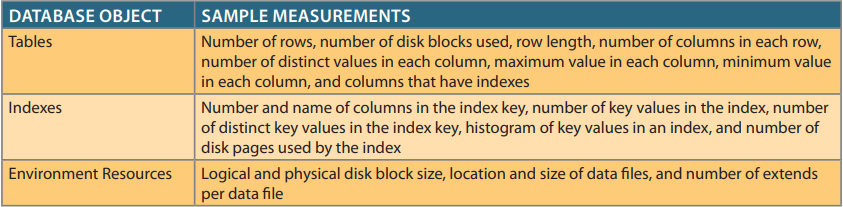
\includegraphics[scale=0.5]{pics/stat}
\end{figure}
\section{Query Processing}
\chapter{Distributed Database Management Systems}
\chapter{SQL Fundamentals 1}
\chapter{SQL Fundamentals 2}
\chapter{Business Intelligence and Data Warehouses}
\chapter{Big Data and NoSQL}
\chapter{Database Administration and Security}
\end{document}